\tableofcontents

\pagebreak

\section{Построение математической модели объекта}
\subsection{Вывод уравнений}
\begin{figure}[h]
    \centering
    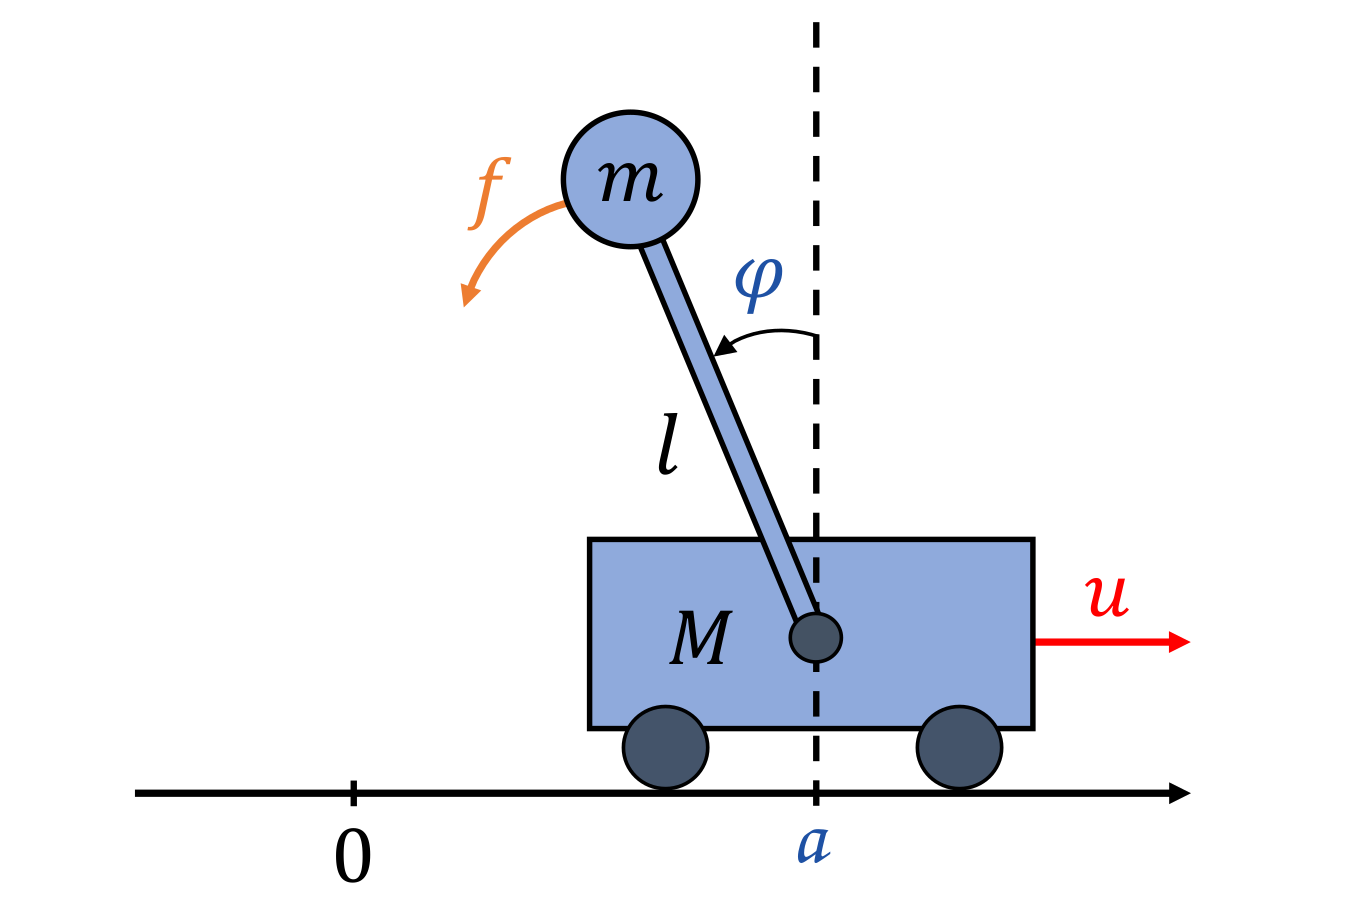
\includegraphics[width=300px]{pendulum.png}
    \caption{\label{fig:task1_1}Перевернутый маятник на тележке.}
\end{figure}

Рассмотрим систему перевернутого маятника на тележке (рис. \ref{fig:task1_1}). Введем следущие обозначения физических величин:
\begin{itemize}
    \item $a$ -- линейная координата тележки;
    \item $\dot{a}$ -- линейная скорость тележки;
    \item $\varphi$ -- угол отклонения маятника от вертикали;
    \item $\dot{\varphi}$ -- угловая скорость маятника;
    \item $f$ -- вращающий внешний момент, действующий на маятник;
    \item $u$ -- сила действующая на тележку;
    \item $M, m$ --  массы тележки и маятника соответственно;
    \item $l$ -- длина маятника.
\end{itemize}

В качестве вектора состояния $x = \begin{bmatrix}
    x_1 & x_2 & x_3 & x_4
\end{bmatrix}^T$ выберем набор $a, \dot{a}, \varphi, \dot{\varphi}$. В роли управляющего воздействия примем $u$, в роли внешнего возмущения -- $f$.
Измеряемыми сигналами $y = \begin{bmatrix}
    y_1 & y_2
\end{bmatrix}^T$ будем считать $a$ и $\varphi$.
\begin{equation} \label{eq:1}
    \begin{cases}
        x_1 = a \\ x_2 = \dot{a} \\ x_3 = \varphi \\ x_4 = \dot{\varphi} \\ y_1 = a \\ y_2 = \varphi
    \end{cases}
\end{equation}

Для вывода математической модели данной физической системы воспользуемся уравнениями Лагранжа:
\begin{equation} \label{eq:2}
    \begin{cases}
        \frac{d}{dt}\frac{\partial T}{\partial \dot{a}} - \frac{\partial T}{\partial a} = u \\
        \frac{d}{dt}\frac{\partial T}{\partial \dot{\varphi}} - \frac{\partial T}{\partial \varphi} = f + mgl\sin(\varphi)
    \end{cases},
\end{equation}
где $T$ -- кинетическая энергия системы.
\begin{equation} \label{eq:3}
    T(t) = M\frac{\dot{a}^2}{2} + m\frac{(\frac{d}{dt}(l\cos(\varphi)))^2 + (-\frac{d}{dt}(l\sin(\varphi)) + \dot{a})^2}{2}=
    (M+m)\frac{\dot{a}^2}{2} + \frac{ml^2\dot{\varphi}^2}{2} - ml\cos(\varphi)\dot{a}\dot{\varphi}
\end{equation}
Подставив выражение для $T$ в уравнения \ref{eq:2}, получим уравнения математической модели системы:
\begin{equation} \label{eq:4}
    \begin{cases}
        (M+m)\ddot{a} + ml(\sin(\varphi)\dot{\varphi}^2 - \cos(\varphi)\ddot{\varphi}) = u \\
        ml^2\ddot{\varphi} - ml\ddot{a}\cos{\varphi} = f + mgl\sin(\varphi)
    \end{cases}
\end{equation}
Тогда, выразив $\ddot{a}$ и $\ddot{\varphi}$:
\begin{equation} \label{eq:5}
    \begin{cases}
        \ddot a = -\frac{ml}{M+m}\sin(\varphi)\dot{\varphi}^2 + \frac{ml}{M+m}\cos(\varphi)\ddot{\varphi} + \frac{1}{M+m}u \\
        \ddot \varphi = \frac{1}{l}\ddot a \cos(\varphi) + \frac{g}{l}\sin(\varphi) + \frac{1}{ml^2}f
    \end{cases}
\end{equation}
Решив данную систему уравнений \ref{eq:5} относительно $\ddot a$ и $\ddot \varphi$:
\begin{equation} \label{eq:6}
    \begin{cases}
        \ddot a = \frac{1}{M + m\sin(\varphi)^2}( -ml\sin(\varphi)\dot{\varphi}^2 + mg\cos(\varphi)\sin(\varphi) + \frac{\cos(\varphi)}{l}f + u ) \\
        \ddot \varphi = \frac{1}{M + m\sin(\varphi)^2}( -m\sin(\varphi)\cos(\varphi)\dot{\varphi}^2 + \frac{(M+m)g}{l}\sin(\varphi) + \frac{M+m}{ml^2}f + \frac{\cos(\varphi)}{l}u )
    \end{cases}
\end{equation}

Представим математическую модель в терминах вектора состояния:
\begin{equation} \label{eq:7}
    \begin{cases}
        \dot x_1 = x_2 \\
        \dot x_2 = \frac{1}{M + m\sin(x_3)^2}( -ml\sin(x_3)x_4^2 + mg\cos(x_3)\sin(x_3) + \frac{\cos(x_3)}{l}f + u ) \\
        \dot x_3 = x_4 \\
        \dot x_4 = \frac{1}{M + m\sin(x_3)^2}( -m\sin(x_3)\cos(x_3)x_4^2 + \frac{(M+m)g}{l}\sin(x_3) + \frac{M+m}{ml^2}f + \frac{\cos(x_3)}{l}u ) \\
        y_1 = x_1 \\
        y_2 = x_3
    \end{cases}
\end{equation}

\subsection{Точки равновесия}
В точках равновесия все компоненты производной вектора состояния по времени равны $0$. Следовательно, полагая $u, f \equiv 0$
необходимо:
\begin{equation} \label{eq:8}
    \begin{cases}
        x_2 = 0 \\
        \frac{1}{M + m\sin(x_3)^2}( -ml\sin(x_3)x_4^2 + mg\cos(x_3)\sin(x_3) ) = 0 \\
        x_4 = 0 \\
        \frac{1}{M + m\sin(x_3)^2}( -m\sin(x_3)\cos(x_3)x_4^2 + \frac{(M+m)g}{l}\sin(x_3) ) = 0 \\
    \end{cases}
\end{equation}
Учитывая $x_4 = 0$ и $M + m\sin(x_3)^2 > 0$:
\begin{equation} \label{eq:9}
    \begin{cases}
        x_1 \in \mathbb{R} \\
        x_2 = 0 \\
        x_3 = \pi n, n \in \mathbb{Z} \\ 
        x_4 = 0 
    \end{cases}
\end{equation}
Заметим, однако, что с физической точки зрения условие $x_3 = \pi n$ эквивалентно $x_3 = 0$ (верхнее положение маятника) или $x_3 = \pi$ (нижнее положение маятника). В дальнейшем нас будет интересовать стабилизация системы около верхенего положения равновесия.

\subsection{Линеаризация}
Для линеаризации системы около векхней точки равновесия ($x = \begin{bmatrix}
    a_0 & 0 & 0 & 0
\end{bmatrix}^T$) представим некоторые функции от компонент вектора состояния в виде ряда Тейлора в данной точке:
\begin{equation*}\sin(x_3) = x_3 + \sum_{n=1}^{\infty}(-1)^n\frac{x_3^{2n+1}}{(2n+1)!}\end{equation*}
\begin{equation*}\cos(x_3) = 1 + \sum_{n=1}^{\infty}(-1)^n\frac{x_3^{2n}}{(2n)!}\end{equation*}
Приняв величины вектора состояния достаточно малыми ($x_3^2 \ll x_3$, $x_4^2 \ll x_4$), можем записать линеаризованные уравненя динамики системы:
\begin{equation} \label{eq:10}
    \begin{cases}
        \dot x_1 = x_2 \\
        \dot x_2 = \frac{mg}{M}x_3 + \frac{1}{Ml}f + \frac{1}{M}u \\
        \dot x_3 = x_4 \\
        \dot x_4 = \frac{(m+m)g}{Ml}x_3 + \frac{M+m}{Mml^2}f + \frac{1}{Ml}u \\
    \end{cases}
\end{equation}

Можем представить линеаризованную систему в матричном виде:
\begin{equation} \label{eq:11}
    \begin{cases}
        \dot x = Ax + Bu + Df \\
        y = Cx
    \end{cases},
\end{equation}
где матрицы $A$, $B$, $C$, $D$ имеют следующий вид:
\begin{equation*}
    A = \begin{bmatrix}
        0 & 1 & 0 & 0 \\
        0 & 0 & \frac{mg}{M} & 0 \\
        0 & 0 & 0 & 1 \\
        0 & 0 & \frac{(M+m)g}{Ml} & 0
    \end{bmatrix},
    B = \begin{bmatrix}
        0 \\ \frac{1}{M} \\ 0 \\ \frac{1}{Ml}
    \end{bmatrix},
    D = \begin{bmatrix}
        0 \\ \frac{1}{Ml} \\ 0 \\ \frac{M+m}{Mml^2}
    \end{bmatrix},
    C = \begin{bmatrix}
        1 & 0 & 0 & 0 \\
        0 & 0 & 1 & 0
    \end{bmatrix}
\end{equation*}

Выберем значения параметров системы:
\begin{equation*}
    M = 10, m = 1, l = 1, g = 9.8
\end{equation*}
Тогда, матрицы системы примут следующий вид:
\begin{equation*}
    A = \begin{bmatrix}
        0 & 1 & 0 & 0 \\
        0 & 0 & 0.98 & 0 \\
        0 & 0 & 0 & 1 \\
        0 & 0 & 10.78 & 0
    \end{bmatrix},
    B = \begin{bmatrix}
        0 \\ 0.1 \\ 0 \\ 0.1
    \end{bmatrix},
    D = \begin{bmatrix}
        0 \\ 0.1 \\ 0 \\ 1.1
    \end{bmatrix},
    C = \begin{bmatrix}
        1 & 0 & 0 & 0 \\
        0 & 0 & 1 & 0
    \end{bmatrix}
\end{equation*}
\pagebreak

\section{Анализ математической модели}
\subsection{Анализ матриц}
Найдем собственные числа и собственные вектора матрицы $A$:
\begin{equation*}
    \sigma(A) = \{0, 0, 3.28, -3.28\}; \nu(A) = \{\begin{bmatrix}
        1 \\ 0 \\ 0 \\ 0
    \end{bmatrix},
    \begin{bmatrix}
        -1 \\ 0 \\ 0 \\ 0
    \end{bmatrix},
    \begin{bmatrix}
        0.026 \\ 0.087 \\ 0.29 \\ 0.953
    \end{bmatrix},
    \begin{bmatrix}
        -0.026 \\ 0.087 \\ -0.29 \\ 0.953
    \end{bmatrix}\}
\end{equation*}
Заметим, что первые два собственных вектора линейно зависимы и соответствуют нулевым собственным числам. Можем сделать вывод,
что первая компонента вектора состояния не влияет на динамику системы (от координаты тележки не зависят другие параметры и их производные).

Имея кратные нулевые корни, а также положительное собственное число, система является неустойчивой. Проведем анализ на управляемость, стабилизируемость, наблюдаемость и обнаруживаемость приведя систему в Жорданов базис:
\begin{equation*}
    A = PJP^{-1} = \begin{bmatrix}
        1 & 0 & -0.03 & 0.03 \\
        0 & 1 & 0.09 & 0.09 \\
        0 & 0 & -0.31 & 0.31 \\
        0 & 0 & 1 & 1
    \end{bmatrix}
    \begin{bmatrix}
        0 & 1 & 0 & 0 \\
        0 & 0 & 0 & 0 \\
        0 & 0 & -3.28 & 0 \\
        0 & 0 & 0 & 3.28
    \end{bmatrix}
    \begin{bmatrix}
        1 & 0 & -0.03 & 0.03 \\
        0 & 1 & 0.09 & 0.09 \\
        0 & 0 & -0.31 & 0.31 \\
        0 & 0 & 1 & 1
    \end{bmatrix}^{-1}
\end{equation*}
\begin{equation*}
    P^{-1}B = \begin{bmatrix}
        0 \\ 0.09 \\ 0.05 \\ 0.05
    \end{bmatrix},
    CP = \begin{bmatrix}
        1 & 0 & -0.03 & 0.03 \\
        0 & 0 & -0.31 & 0.31
    \end{bmatrix}
\end{equation*}
Можем сделать вывод, что система является полностью управляемой и наблюдаемой (соответственно стабилизируемой и обнаруживаемой).

\subsection{Передаточные функции}
Найдем передаточные матрицы системы от входа к выходу и от внешнего возмущения к выходу:
\begin{equation*}
    \underset{u\to y}{W}(s) = \begin{bmatrix}
        \frac{0.1s^2 - 0.98}{s^4 - 10.78s^2} \\
        \frac{0.1}{s^2 - 10.78}
    \end{bmatrix}, 
    \underset{f\to y}{W}(s) = \begin{bmatrix}
        \frac{0.1}{s^2 - 10.78} \\
        \frac{1.1}{s^2 - 10.78}
    \end{bmatrix}
\end{equation*}
Динамический порядок функции $\frac{0.1s^2 - 0.98}{s^4 - 10.78s^2}$ равен $4$, для остальных -- $2$. Относительный динамический порядок всех функций равен $2$.
Нули присутствуют только у функции $\frac{0.1s^2 - 0.98}{s^4 - 10.78s^2}$ и равны $\pm 3.13$. Полюса передаточных функций соответствуют собственным числам матрицы динамики системы.

Все функции описывают расходящийся переходный процесс при нулевом входном (внешнем) воздействии, т.к. имеют кратные нулевые или положительный полюса.

\subsection{Линейное моделирование}
Выполним моделирование линеаризованной системы, заданной уравнениями \ref{eq:11}.
Ниже приведены графики, демонстрирующие динамику вектора состояния при различных начальных условиях.

\begin{figure}[]
    \centering
    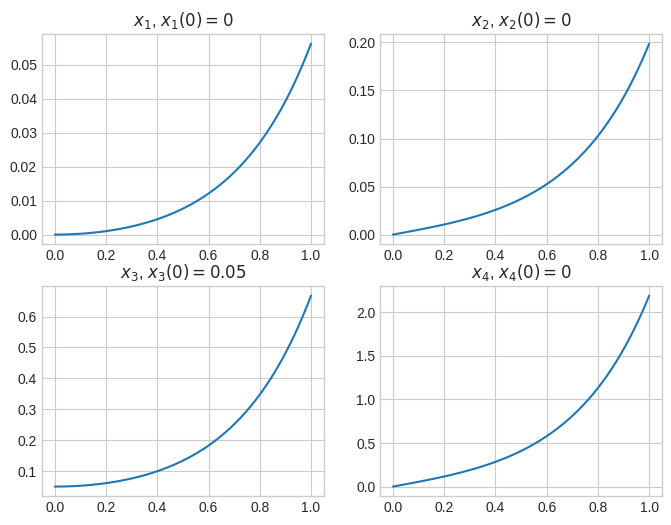
\includegraphics[width=300px]{state_lin_1.png}
    \caption{\label{fig:task2_3_1}Моделирование линеаризованной системы ($x(0)=\begin{bmatrix}
        0 & 0 & 0.05 & 0
    \end{bmatrix}^T$).}
\end{figure}

\begin{figure}[]
    \centering
    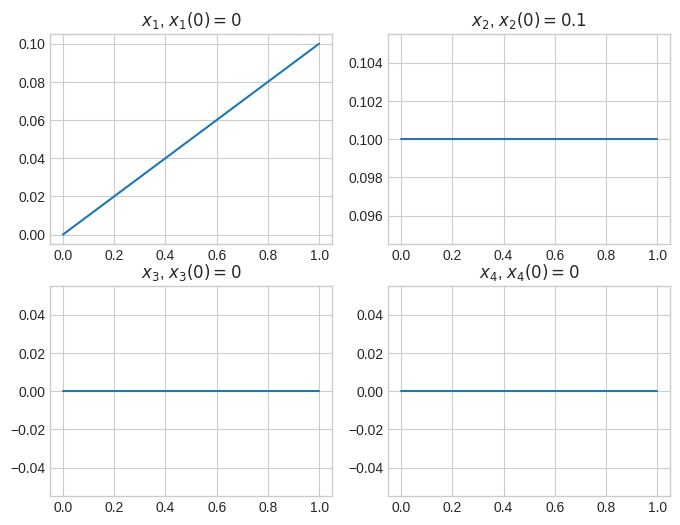
\includegraphics[width=300px]{state_lin_2.png}
    \caption{\label{fig:task2_3_2}Моделирование линеаризованной системы ($x(0)=\begin{bmatrix}
        0 & 0.1 & 0 & 0
    \end{bmatrix}^T$).}
\end{figure}

\begin{figure}[]
    \centering
    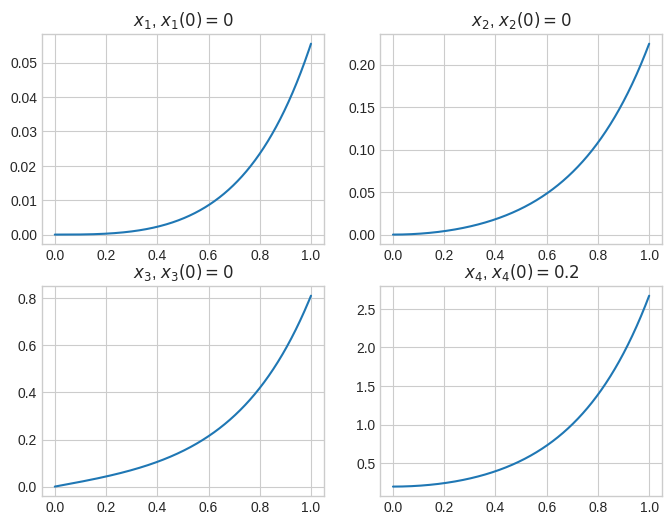
\includegraphics[width=300px]{state_lin_3.png}
    \caption{\label{fig:task2_3_3}Моделирование линеаризованной системы ($x(0)=\begin{bmatrix}
        0 & 0 & 0 & 0.2
    \end{bmatrix}^T$).}
\end{figure}

\begin{figure}[]
    \centering
    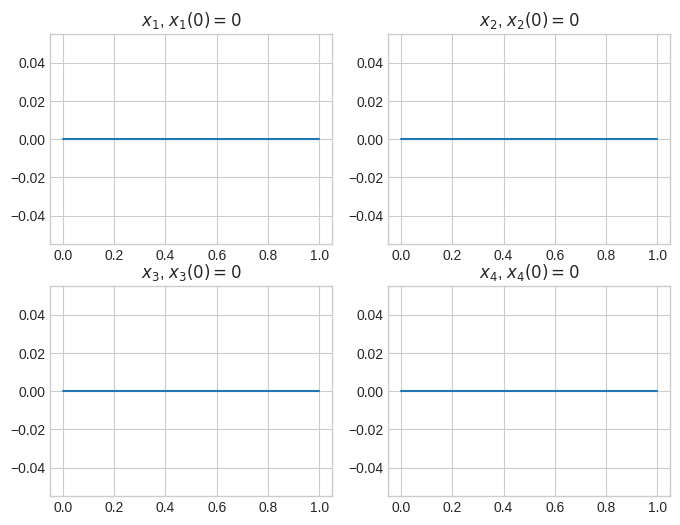
\includegraphics[width=300px]{state_lin_4.png}
    \caption{\label{fig:task2_3_4}Моделирование линеаризованной системы ($x(0)=\begin{bmatrix}
        0 & 0 & 0 & 0
    \end{bmatrix}^T$).}
\end{figure}

\subsection{Нелинейное моделирование}
Выполним моделирование исходной системы, заданной уравнениями \ref{eq:7}.
Ниже приведены графики, демонстрирующие динамику вектора состояния при различных начальных условиях.

\begin{figure}[h]
    \centering
    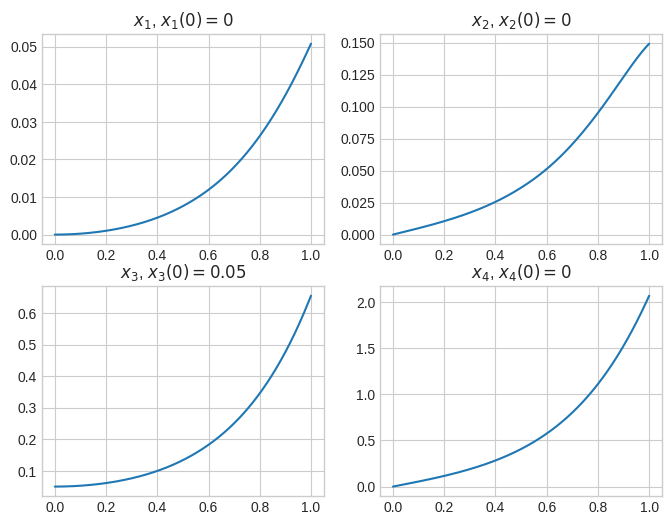
\includegraphics[width=300px]{state_nonlin_1.png}
    \caption{\label{fig:task2_4_1}Моделирование исходной системы ($x(0)=\begin{bmatrix}
        0 & 0 & 0.05 & 0
    \end{bmatrix}^T$).}
\end{figure}

\begin{figure}[]
    \centering
    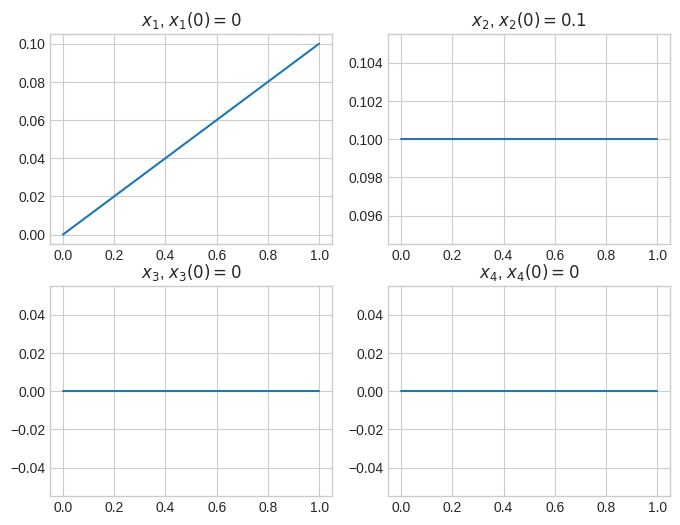
\includegraphics[width=300px]{state_nonlin_2.png}
    \caption{\label{fig:task2_4_2}Моделирование исходной системы ($x(0)=\begin{bmatrix}
        0 & 0.1 & 0 & 0
    \end{bmatrix}^T$).}
\end{figure}

\begin{figure}[]
    \centering
    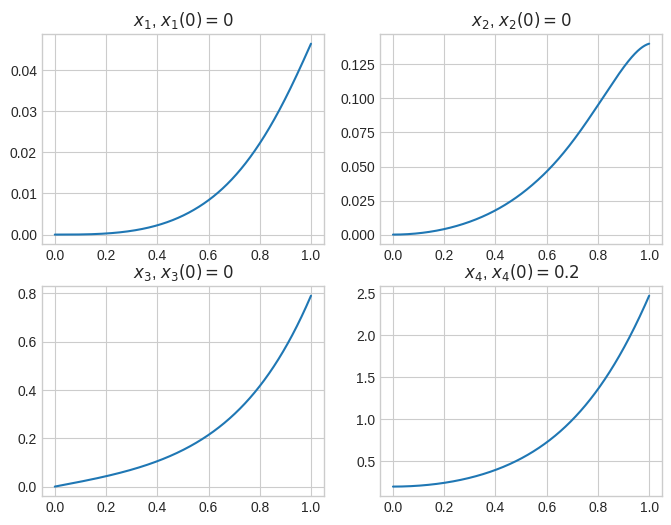
\includegraphics[width=300px]{state_nonlin_3.png}
    \caption{\label{fig:task2_4_3}Моделирование исходной системы ($x(0)=\begin{bmatrix}
        0 & 0 & 0 & 0.2
    \end{bmatrix}^T$).}
\end{figure}

\begin{figure}[]
    \centering
    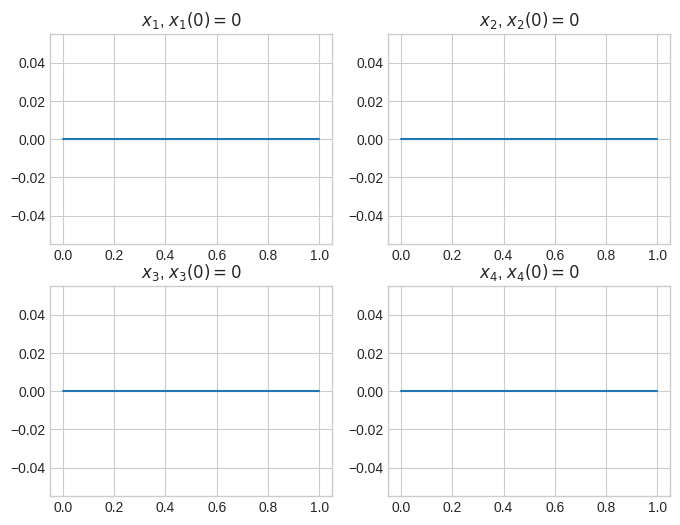
\includegraphics[width=300px]{state_nonlin_4.png}
    \caption{\label{fig:task2_4_4}Моделирование исходной системы ($x(0)=\begin{bmatrix}
        0 & 0 & 0 & 0
    \end{bmatrix}^T$).}
\end{figure}
\pagebreak
Заметим, что при малом времени моделирования динамика систем очень схожая. Построим сравнительные графики при большем времени переходного процесса.

\begin{figure}[]
    \centering
    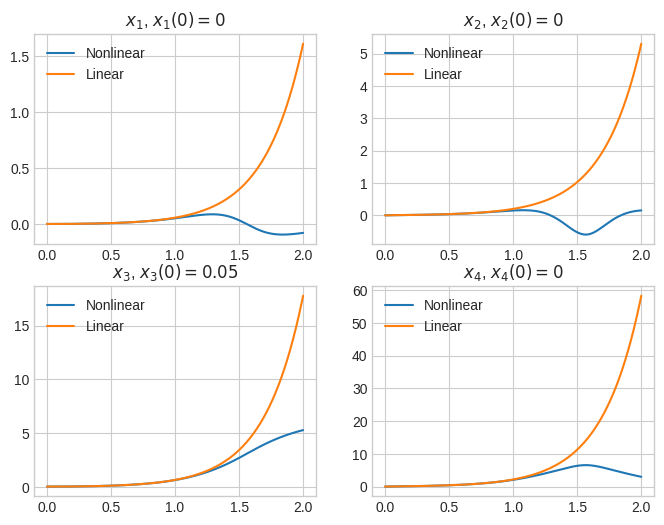
\includegraphics[width=300px]{state_lin_nonlin_1.png}
    \caption{\label{fig:task2_4_5}Сравнительное моделирование систем ($x(0)=\begin{bmatrix}
        0 & 0 & 0.05 & 0
    \end{bmatrix}^T$).}
\end{figure}

\begin{figure}[]
    \centering
    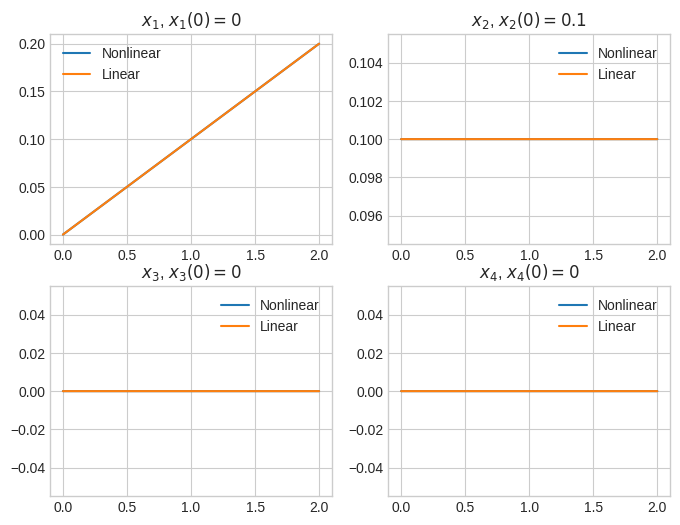
\includegraphics[width=300px]{state_lin_nonlin_2.png}
    \caption{\label{fig:task2_4_6}Сравнительное моделирование систем ($x(0)=\begin{bmatrix}
        0 & 0.1 & 0 & 0
    \end{bmatrix}^T$).}
\end{figure}

\begin{figure}[]
    \centering
    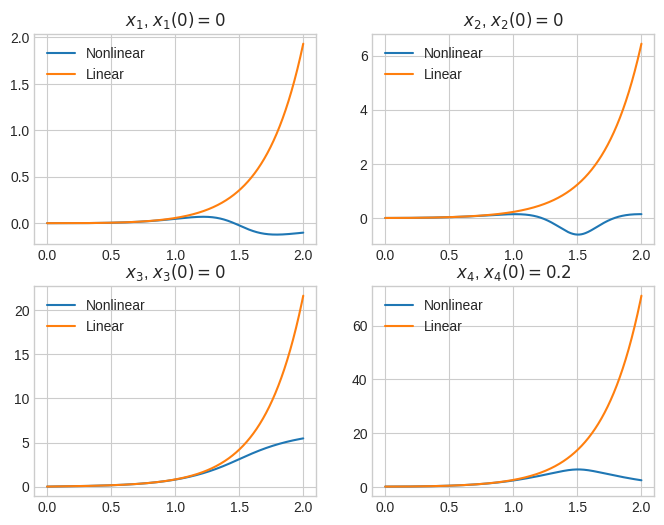
\includegraphics[width=300px]{state_lin_nonlin_3.png}
    \caption{\label{fig:task2_4_7}Сравнительное моделирование систем ($x(0)=\begin{bmatrix}
        0 & 0 & 0 & 0.2
    \end{bmatrix}^T$).}
\end{figure}

\begin{figure}[]
    \centering
    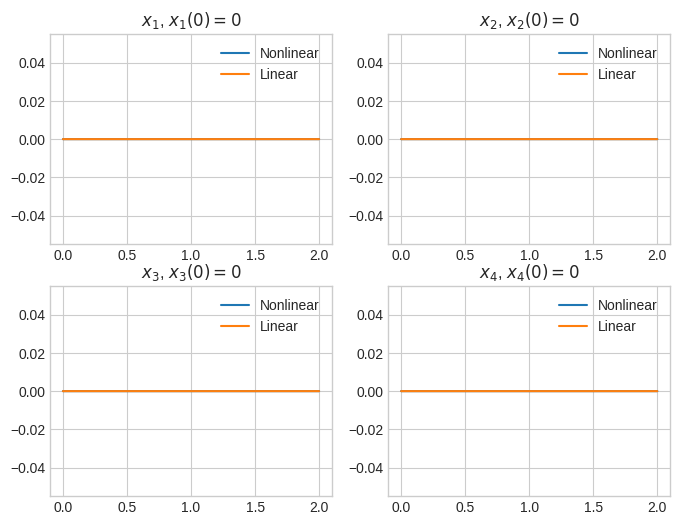
\includegraphics[width=300px]{state_lin_nonlin_4.png}
    \caption{\label{fig:task2_4_8}Сравнительное моделирование систем ($x(0)=\begin{bmatrix}
        0 & 0 & 0 & 0
    \end{bmatrix}^T$).}
\end{figure}

\pagebreak
При увеличении времени моделирования расхождения становятся явно заметными.

\section{Модальное управление}
\pagebreak

\section{Регуляторы с заданной степенью устойчивости}